\chapter{Implementación}

Para la implementación de la solución utilizaremos una arquitectura cliente-servidor\cite{client-server}, la cual nos
permite tener los datos centralizados en una aplicación servidor. La aplicación cliente realizará peticiones al
servidor, para que este le provea de los datos que necesite en cada momento.\\

\section{Servidor}
En el lado del servidor o \textit{back-end} se encuentra la mayor parte de la lógica de la aplicación, dedicándose el
lado del cliente a simplemente mostrarla en una interfaz cómoda para el usuario.\\

Se ha implementado un servidor que provee a los clientes de un listado de series y sus temporadas, así como de la
posibilidad de crear reseñas de las mismas o obtener las reseñas de otros usuarios.

\subsection{Lenguaje de programación}
El lenguaje de programación seleccionado para el servidor es \textit{Python}\cite{python}, ya que es un lenguaje de
programación que nos provee de una buena experiencia de desarrollo al ser un lenguaje menos estricto y cuenta con muchas
librerías útiles y una enorme comunidad a sus espaldas.\\

Uno de sus puntos débiles, es que al ser un lenguaje no tipado, es más propenso a errores de sintaxis, pero desde la
versión 3.5, cuenta con una forma de tipar el código, de forma que, aunque el intérprete de \textit{Python} no detecte
este tipado, puede ser utilizado por herramientas de los \textit{IDEs} y \textit{linters} para la detección precoz
errores.\\

Otro de los motivos que me han llevado a decantarme por este lenguaje son sus librerías científicas y de procesamiento
de datos. Con ellas, en un futuro podríamos incluir en la aplicación alguna herramienta para obtener estadísticas y
realizar predicciones sobre nuestros datos. Algo muy útil para un cliente que quiera usar los datos de la aplicación
para saber qué tipo de series interesan a cierto tipo de público, por ejemplo.\\

Como gestor de paquetes y dependencias, utilizo \textit{poetry}\cite{poetry}, que nos permite gestionar las dependencias
del proyecto de forma muy sencilla y similar a \textit{NPM}\cite{npm}.

\subsection{Framework}
El framework utilizado para el servidor es \textit{Flask}\cite{flask}, un framework de Python que nos permite una 
\textit{REST API}\cite{rest} minimalista, flexible y fácil de usar.

\subsection{Operaciones}
Recopilación y breve descripción de las peticiones que atiende el servidor.

\subsubsection{Listado y detalles de series}
El servidor provee de una lista de series o de los detalles de una serie en particular a través de su identificador. Sin
embargo, la base de datos no incluye la información de estas series, si no que se obtienen a través de una API
externa.\\

La API utilizada es \textit{TheMovieDB}, una API abierta que provee de datos sobre series y películas. En este caso,
haremos uso de las series. Gracias al diseño de nuestra aplicación, podríamos cambiar de API en cualquier momento, sin
que suponga mucho tiempo de desarrollo.

\subsection{Test}
Como ya hablamos en la \hyperref[chap:metodología]{metodología}, necesitamos que el código cumpla con unos requisitos
mínimos de calidad a través de \textit{tests}.\\

Para el servidor, se han implementado tests unitarios con la librería \textit{pytest}\cite{pytest}, que comprueban que
los métodos de los modelos de la aplicación funcionan correctamente.
\begin{figure}[H]
\centering	
    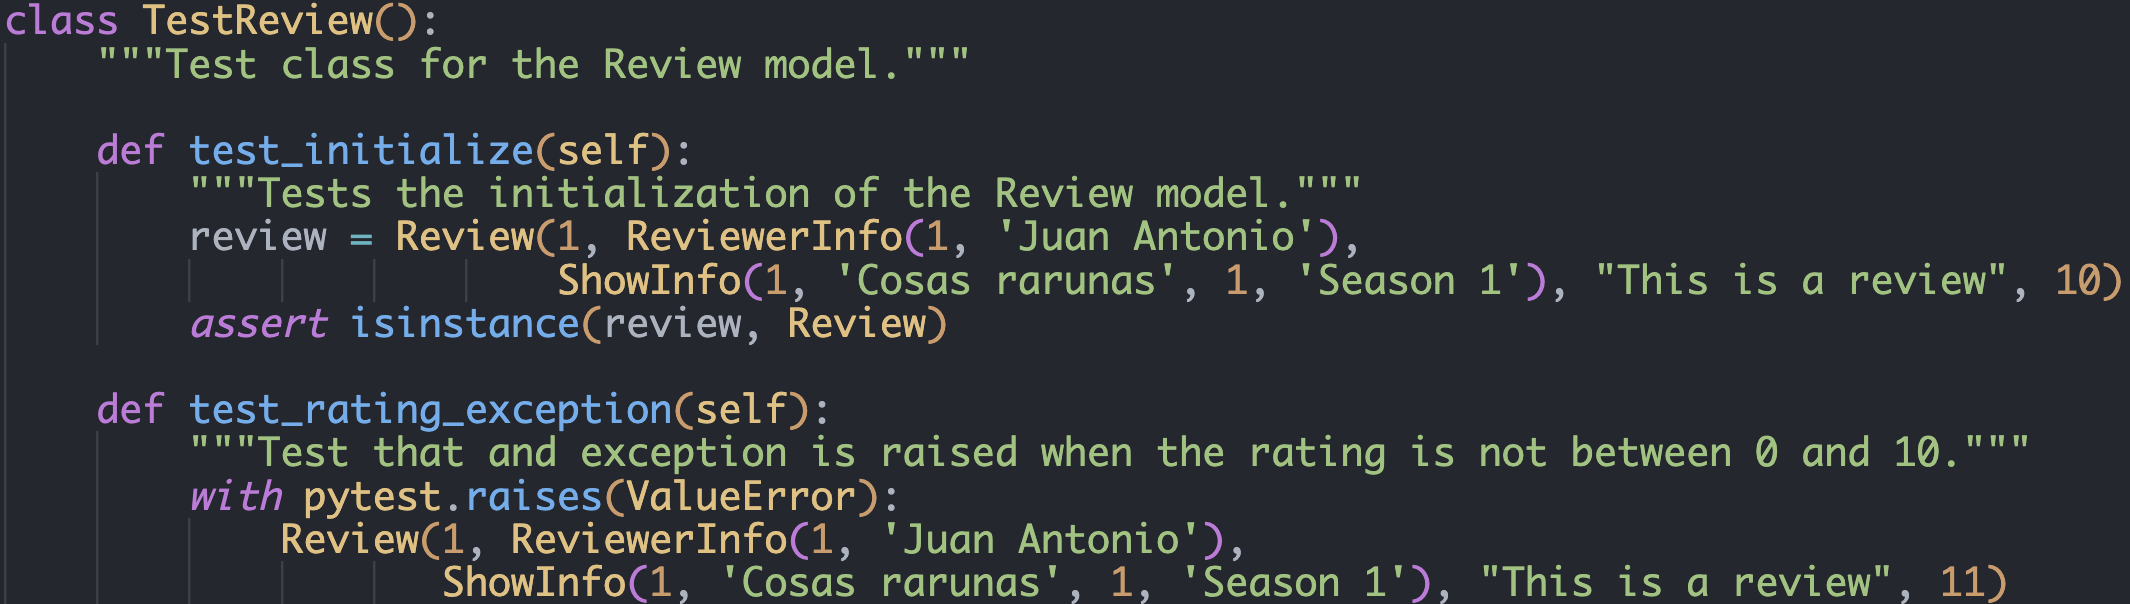
\includegraphics[scale=0.25]{img/pytest.png}
\caption{ Test unitario de la clase Show en Python }\label{fig:pytest}
\end{figure}

\subsection{Base de datos}
El número de reseñas irá en aumento con el tiempo y con el número de usuarios de la aplicación, por lo que necesito una
base de datos que sea fácilmente escalable. Por ello, \textit{MongoDB}\cite{mongodb} es una muy buena opción, gracias a
\textit{MongoAtlas}\cite{mongoatlas}, una herramienta \textit{DataBase as a Service}\cite{dbaas} que nos permite escalar
la base de datos verticalmente, aumentando el poder de procesamiento de nuestro cluster, u horizontalmente, añadiendo
más nodos para compartir la carga.\\

Además, guarda los datos en formato \textit{JSON}\cite{json}, lo que nos permite acceder a ellos de forma muy sencilla y
fácilmente interpretable por cualquier lenguaje de programación moderno.

\subsection{Configuración}

Las variables de configuración se encuentran en los ficheros del directorio \textit{config} y se definen mediante las
variables de entorno, incluyendo opciones por defecto en la mayoría. En el entorno de desarrollo, uso \textit{dotenv}
para cargar las variables de entorno desde un fichero de configuración \textit{.env}.
\begin{figure}[H]
\centering	
    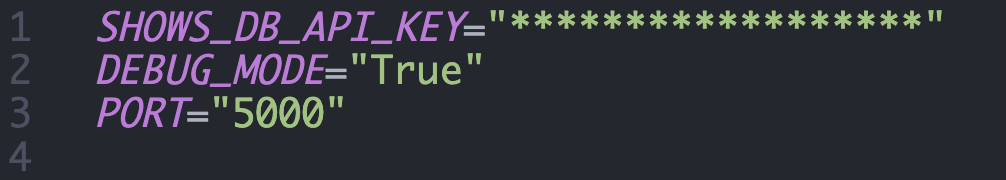
\includegraphics[scale=0.525]{img/dotenv.png}
\caption{ Fichero de configuración con las variables de entorno del servidor }\label{fig:dotenv}
\end{figure}
